% Prof. Dr. Ausberto S. Castro Vera
% UENF - CCT - LCMAT - Curso de Ci\^{e}ncia da Computa\c{c}\~{a}o
% Campos, RJ,  2015
% Disciplina: An\'{a}lise e Projeto de Sistemas
% Aluno: Rodolfo Gomes Peixoto


\chapter{Etapa de An\'{a}lise}
Os requisitos são caracteristicas, atributos e habilidade que um sistema deve conter para que seja um software
para aquele determinado serviço ou produto.
  \section{Requisitos do sistema}
 \subsection{Requisitos}
  \begin{enumerate}
      \item Servidor
      \item Rede de Computadores
      \item Cabos de rede
      \item Estabilizador
      \item No-break
      \item Sistema Operacional
      \item Linguagem Orientada a Objeto
      \item Interface Gráfica
      \item Pré-matrícula
      \item Leitor de PDF
      \item Cadastro de Alunos
      \item Cadastro de Professores
      \item Cadastro de Matérias
      \item Cadastro de Notas
      \item Exclusão de disciplinas
      \item Inclusão de Disciplinas
      \item Roteadores
      \item Manual do Sistema Operacional
      \item Relatórios
      \item Trancamento da Matrícula
      \item Trancamento de Disciplinas
      \item Registrar Log para cada usuário
      \item Backup do Sistema
      \item Treinamento dos Alunos
      \item Treinamento dos Professores
      \item Treinamento dos Funcionários
      \item Operador de Rede
      \item Página Web
      \item Segurança do Servidor
      \item Acesso ao Sistema
  \end{enumerate}
  
  \subsection{Definição}
  \begin{enumerate}
\item O sistema deve ter um servidor onde esta o aplicativo.
\item O sistema deve ter uma rede de computadores robusta com dois links de rede.
\item A rede do sistema deve  funcionar usando cabeamento.
\item Os estabilizadores devem evitar que os picos de energia afete as componentes de hardware do sistema.
\item O no-break deverá armazenar energia até que possa desligar o servidor com segurança.
\item O servidor deverá conter um sistema operacional para gerenciar as componentes de software e hardware.
\item Os módulos do sistema deverão ser criados com uma linguagem de programação orientada a objeto.
\item O sistema deverá conter uma interface agradável e iterativa para que o usuário possa facilmente utilizar.
\item O sistema conterá um sistema de pré-matrícula para automatizar e diminuir o uso de papel.
\item O sistema permitirá a leitura de arquivos PDFs.
\item Os alunos terão um cadastro na qual poderão acessar seus dados.
\item Os professores terão acesso a uma área restrita.
\item  O sistema deve conter as notas dos alunos para maior facilidade
\item Haverá a possibilidade de visualizar as notas de todas as matérias já cursadas e em andamento.
\item Os alunos também terão a opção de fazer a exclusão das disciplinas
\item Os alunos poderão fazer a inclusão de disciplina pelo sistema.
\item O sistema deve utilizar roteadores para acessarem a rede local.
\item O sistema deve conter o manual para maior facilidade de acesso.
\item Os relatórios são importantes para que seja feito o acompanhamento de como o sistema está funcionando.
\item O aluno pode fazer o trancamento da matrícula.
\item O trancamento de disciplinas pode ser feito caso o aluno desista da disciplina.
\item O acesso ao sistema deve ser feito utilizando matrícula e senha.
\item Salvar as informações do sistema periodicamente.
\item Deve ser executado o treinamento de todo o pessoal do sistema.
\item O treinamento será on-line.
\item O treinamento será diferenciado.
\item O sistema deve ter um operador de rede para fazer a manutenção e acesso.
\item Deve permitir o acesso a informações básicas da instituição de ensino para consulta dos usuários.
\item A Segurança do Site garante sigilo dos dados do cliente.
\item É necessário para que o serviço de atendimento esteja em operação.

  \end{enumerate}
   
 \subsection{Especificação dos Requisitos}
   \begin{itemize}
   \item Trancamento de Matrícula 
	\begin{itemize}
	\item Deverá ser inserido os dados do aluno pelo funcionário
	\item Terá uma interface gráfica 
	\item Deve estar em dia com a biblioteca.
	\item Nenhum documento pode estar pendente.
	\item O aluno, responsável(caso seja menor de idade) ou outra pessoa portando 
	\end{itemize}
\item Inclusão de Disciplinas
	\begin{itemize}
	\item Não pode estar matriculado em outra matéria no mesmo horário e dia.
	\item Deve estar sem requisito.
	\item A disciplina deve ser do período correspondente.
	\item Deve ser verificada se a disciplina é obrigatória, optativa ou eletiva.
	\end{itemize}
\item Rede de Computadores
	\begin{itemize}
	\item Os roteradores deverão ser instalados
	\item Os cabos deverão ser conectados aos roteadores.
	\item Devera ter uma conexao de internet propria.
	\item É oferecido acesso rápido a informações sobre o atendimento
	\item Ingressar informações de acesso (matrícula, senha) 
	\item Verificar usuário cadastrado 
	\item Verificar senha cadastrada 
	\item Liberar perfil de usuário 
	\item Liberar área e ferramentas de trabalho
	\item Clicar no ícone de chamadas
	\item Confirmar dados pessoais e endereço
	\item Acessar pagamento via boleto bancário ou cartão de crédito
	\item Haverá uma rede interna separada do servidor para a utilização em computadores locais.
	\item Verificar se o software do roteador gera relatórios de picos de rede.
	\end{itemize}
\item Acesso ao sistema
	\begin{itemize}
	\item Ligar o computador
	\item interface grafica
	\item Verificar acesso à Internet
	\item Verificar funcionário cadastrado 
	\item Verificar senha cadastrada 
	\item Liberar perfil de funcionário 
	\item Liberar área e ferramentas de trabalho
	\end{itemize}
\item Exclusão de Disciplinas
	\begin{itemize}
	\item Pode ser feito na data agendada no calendário.
	\item Não será permitido fora do prazo.
	\item O aluno não pode ter abandonado a disciplina.
	\end{itemize}
\item Acesso ao Sistema
	\begin{itemize}
	\item Abrir janela inicial com interface de acesso 
	\item Ingressar informações de acesso (usuário, senha) 
	\item Verificar aluno cadastrado 
	\item Verificar senha cadastrada 
	\item Liberar perfil do aluno 
	\item Liberar área e ferramentas de trabalho 
	\item Permitir acesso à Internet 
	\item Ver relação de chamadas
	\item Finalizar processo
	\end{itemize}
\item Segurança do Servidor
	\begin{itemize}
	\item Sempre atualizar o servidor
	\item Instalar ferramentas de detecção de invasão
	\item O servidor armazena arquivos de diversos usuários
	\item O usuário deve escolher senhas fortes
	\item O sistema é configurado para só aceitar senhas que tenham, por exemplo, um número de caracteres maior do que 8, que sejam por símbolos especiais, dígitos numéricos e caracteres alfabéticos, etc.
	\item Manter o sistema operacional atualizado
	\item Configurar e manter logs atualizados
	\end{itemize}
\item Treinamento dos Alunos
	\begin{itemize}
	\item Será on-line.
	\item A cada seis meses será feito um novo treinamento mostrando as modificações do sistema.
	\item O treinamento terá um prazo específico para o mesmo.
	\item Cada usuário deve ter um treinamento diferenciado
	\end{itemize}
\item Operador de Rede
	\begin{itemize}
	\item A manutenção da rede será feita periodicamente.
	\item O operador pode ser acionado em qualquer momento do dia caso aconteça algum erro.  
	\end{itemize}
\item Manual do Sistema Operacional
	\begin{itemize}
	\item Deve dar aos usuários as instruções para que o acesso seja mais simples.
	\item Deve ser bem detalhado.
	\item Contém ilustrações para maior facilidade de entendimento.
	\item Deve ter cinco idiomas padrão (português, inglês, espanhol, alemão e francês).
	\end{itemize}
  \end{itemize}

   \subsection{Requisitos de Rede}
     \begin{itemize}
     \item	O sistema realizará todo o processo de agendamento e organização visando otimizar o tempo.
     \item	Deverá ser usada para o desenvolvimento do programa a programação estruturada.
     \item	O sistema deverá ter suporte a caracteres especiais característicos da língua portuguesa.
     \item	Os usuários do sistema terão acesso ao sistema apenas por meio da interface gráfica desenvolvida para o tipo mais comum de usuário do serviço realizado pela empresa.
     \item	As páginas da web deverão ter claramente a data da criação e/ou modificação
     \item	A linguagem utilizada para a criação do programa deverá possuir um alto grau de transportabilidade.
     \end{itemize}
        
 
     \subsection{Requisitos de Subsistema}
      \begin{itemize}
      \item	O Sistema deverá suportar o funcionamento de 24 horas continuas para que o site não saia do ar e possa sempre ficar disponível para o agendamento de serviço.
      \item	O Sistema deverá possuir roteadores e switch no padrão internacional com o objetivo de evitar problemas óbvios de compatibilidade.
      \item	Deverá possuir um sistema de impressão compartilhado em rede para maior agilidade do serviço.
      \item	A velocidade de transmissão de dados do sistema deverá opera sob o sistema FastEthernet para garantir sua agilidade e eficiência.
      \item	É também de suma importância que cada subsistema tenha seu próprio backup físico para garantir à segurança dos dados do servidor, diminuindo o máximo possível a perda dos registros por meios de danos físicos causados por fatores externos.
      \end{itemize}

     \subsection{Definições}
       \begin{itemize}
        \item Funcionais
           \begin{itemize}
            \item O sistema deverá conter computadores robustos, pois armazenará todo os dados em um cloud, próprio.
            \item O sistema deverá se comunicar com rapidez e eficiência.
            \item O sistema deverá fazer o cadastro de todas as pessoas que terão acesso ao sistema por meio de uma matrícula.
            \item O servidor deverá monitorar e enviar emails para o administrado em caso de falha, podendo o usuário fazer sugestões e reclamações.
	        \item Monitoramento das notas dos alunos por meio de boletim.
           \end{itemize}
           
         \item Não funcionais
           \begin{itemize}
            \item O sistema utilizará o sistema operacional Linux.
            \item Manutenção Semanal.
            \item Um sistema com várias requisições simultâneas.
            \item Sistema com designer adaptavel para smartphone.
            \item Cada usuário terá o seu tipo de acesso.
           \end{itemize}

        \item Características não desejáveis
	 \begin{itemize}
	        \item Queda do sistema
			\item Poucas pessoas utilizando o sistema.
	     	\item Baixa qualidade do sistema
	 		\item Indisponibilidade do sistema.
	 \end{itemize}
	 
	 \item Do produto
	 \begin{itemize}
	        \item Resultado satisfatório
	 		\item Produtividade dos funcionários
	 		\item Bom desempenho dos funcionários
	  		\item Automatização das funções
	  		\item Diminuição do uso do papel
	  		\item Agilidade ao fazer as matrículas
	  		\item Automatização das informações do meio academico
	 \end{itemize} 
	 
	 \item Da organização
	   \begin{itemize}
	   	    \item Diminuição dos papeis
	        \item Rapidez no serviço.
	    	\item Automatização das tarefas.
	    	\item Eficiência do serviço.
	    	\item Comprimento do prazo combinado
	   \end{itemize} 
	   
	 \item Segurança
	   \begin{itemize}
	   		\item	Firewall deve está atualizado 
	   		\item	A sala do servidor deve conter duas portas com biometria
	   		\item	Interoperabilidade do sistema
	   		\item	Os dados devem ser criptografados
	   		\item	Estabilidade do site
	   \end{itemize}
	   
	     \begin{figure}[H]
	      \centering
	       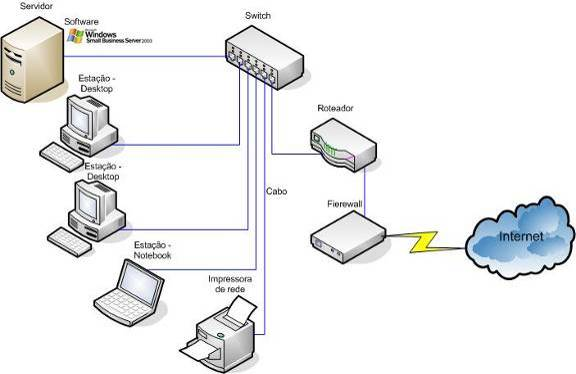
\includegraphics{rede}
	       \caption{Funcionamento da Rede}
	       \label{figRotulo}
               \end{figure}

	   
       \end{itemize}